\section{Results}
The final part was as shown in Fig. \ref{fig:edm}.
\begin{figure}[!htb]%
	\centering
	\subfloat[\centering Detailed CAD View]{{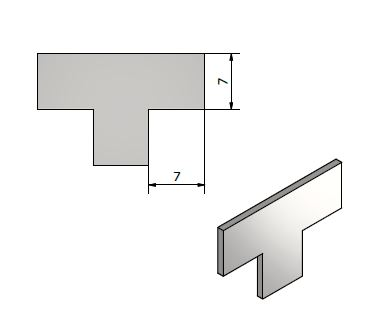
\includegraphics[width=6cm]{Figures/edm cut} }}%
	\qquad
	\subfloat[\centering Final Part]{{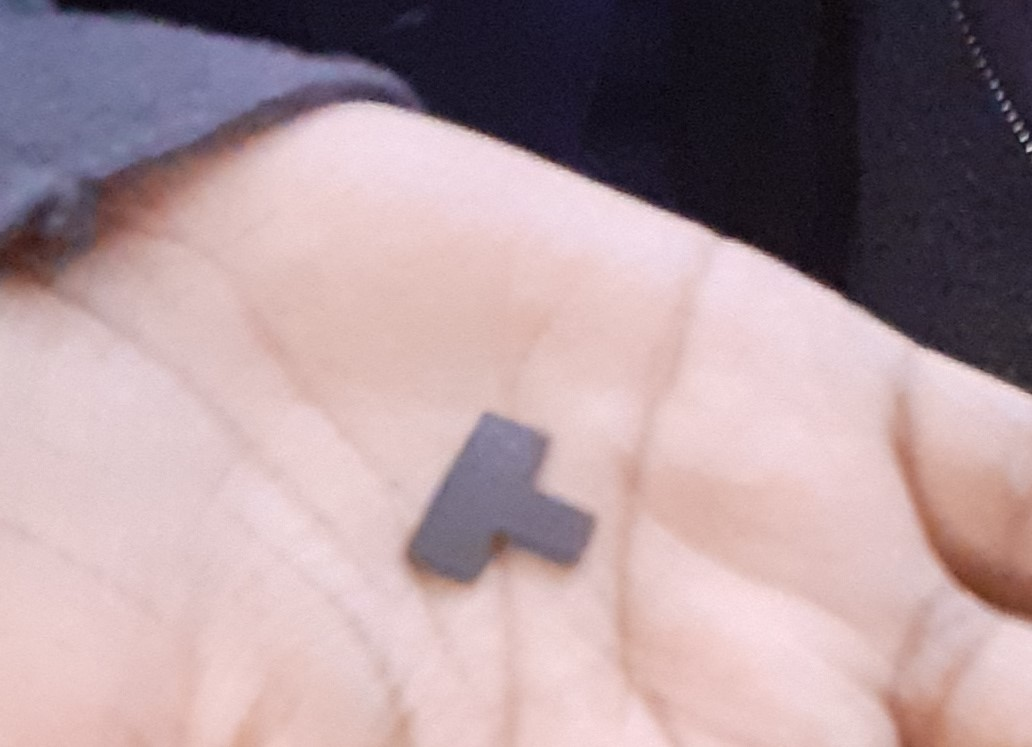
\includegraphics[width=6cm]{Figures/30}}}
	\caption[Final part]{Part cut using Wire EDM}%
	\label{fig:result}%
\end{figure}
\paragraph{}

The code to generate the part was written manually i.e. manual part programming using G- and M- codes specific to the Wire EDM at ENW04 in JKUAT. The list of the G- and M-codes is included in the appendix.